\documentclass{article}


\usepackage{tikz,latexsym}



\usetikzlibrary{arrows,decorations.pathmorphing,decorations.pathreplacing,backgrounds,positioning,fit,matrix}
\usetikzlibrary{shapes,calc,patterns,arrows.meta}
\tikzset{
	vert/.style={circle,inner sep=1.5,fill=white,draw,minimum size=.3cm},
	edge/.style={color=black, thick},
	diredge/.style={->,>={Stealth[width=8pt,length=8pt]},color=black, thick},
	timelabel/.style={fill=white,font=\footnotesize, text centered},
	wave/.style={decorate,decoration={coil,aspect=0}},
	dirwave/.style={->, >={Stealth[width=8pt,length=8pt]},decorate,decoration={coil,aspect=0}},
	diredge2/.style={->,>={Stealth[width=8pt,length=8pt]}}
}
%\tikzstyle{wave} = [decorate,decoration={coil,aspect=0}]
%\tikzstyle{dirwave} = [-{Latex[length=2.5mm]},decorate,decoration={coil,aspect=0}]
%\tikzstyle{diredge2} = [-{Latex[length=2.5mm]}]

\usepackage{caption} %for subfigure - join multiple figures and add captions
\usepackage{subcaption}

\begin{document}
\begin{figure}
	\centering
	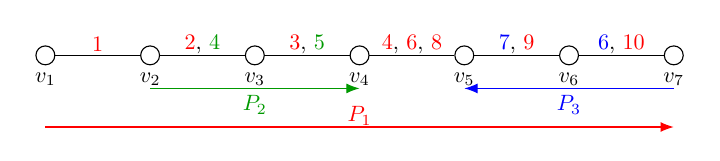
\begin{tikzpicture}[scale = 0.7, every node/.style={scale=0.8},xscale=.95]
		% Variables for distances 
		\def\x{2} % Nodes are \x apart
		\def\y{0.2} % Labels are at distance 0.5 * \x between nodes and \y vertically from the line
		\def\gr{green!60!black}
		\def\bl{blue}
		\def\rd{red}
		
		\node[vert,label=below:$v_1$] (V1) at (1,0) {};
		\node[vert,label=below:$v_2$] (V2) at ($ (V1) + \x*(1,0)$) {};
		\node[vert,label=below:$v_3$] (V3) at ($ (V2) + \x*(1,0)$) {};
		\node[vert,label=below:$v_4$] (V4) at ($ (V3) + \x*(1,0)$) {};
		\node[vert,label=below:$v_5$] (V5) at ($ (V4) + \x*(1,0)$) {};
		\node[vert,label=below:$v_6$] (V6) at ($ (V5) + \x*(1,0)$) {};
		\node[vert,label=below:$v_7$] (V7) at ($ (V6) + \x*(1,0)$) {};
		
		\path[draw] (V1) --(V2);
		\node at ($ (V1) + 0.5*\x*(1,0) + \y*(0,1)$) {{\color{\rd}$1$}};
		\path[draw] (V2) --(V3);
		\node at ($ (V2) + 0.5*\x*(1,0) + \y*(0,1)$) {{\color{\rd}$2$}, {\color{\gr}$4$}};
		\path[draw] (V3) --(V4);
		%\node at ($ (V3) + 0.5*\x*(1,0) + \y*(0,1)$) {{\color{\rd}$3$}, {\color{\gr}$5$},  {\color{\rd}$6$}};
		\node at ($ (V3) + 0.5*\x*(1,0) + \y*(0,1)$) {{\color{\rd}$3$}, {\color{\gr}$5$}};
		\path[draw] (V4) --(V5);
		%\node at ($ (V4) + 0.5*\x*(1,0) + \y*(0,1)$) {{\color{\rd}$4$}, {\color{\rd}$8$}};
		\node at ($ (V4) + 0.5*\x*(1,0) + \y*(0,1)$) {{\color{\rd}$4$}, {\color{\rd}$6$}, {\color{\rd}$8$}};
		
		\path[draw] (V5) --(V6);
		%\node at ($ (V5) + 0.5*\x*(1,0) + \y*(0,1)$) {{\color{\bl}$6$}, {\color{\rd}$9$}};
		\node at ($ (V5) + 0.5*\x*(1,0) + \y*(0,1)$) {{\color{\bl}$7$}, {\color{\rd}$9$}};
		\path[draw] (V6) --(V7);
		%\node at ($ (V6) + 0.5*\x*(1,0) + \y*(0,1)$) {{\color{\bl}$5$}, {\color{\rd}$10$}};
		\node at ($ (V6) + 0.5*\x*(1,0) + \y*(0,1)$) {{\color{\bl}$6$}, {\color{\rd}$10$}};
		
		%\draw[->] ($ (V1) + 2 * \yy * (0,1)$) -- ($ (V7) + 2 * \yy * (0,1)$);
		
		\draw[-Latex,color=\rd] ($(V1) - (0,1.3)$) -- ($ (V7) - (0,1.3)$);
		\node at ($(V4) -(0,1.1)$) {\color{\rd}$P_1$} {};
		\draw[-Latex,color=\gr] ($(V2) - (0,0.6)$) -- ($ (V4) - (0,0.6)$);
		\node at ($(V3) -(0,0.9)$) {\color{\gr}$P_2$} {};
		\draw[-Latex,color=\bl] ($(V7) - (0,0.6)$) -- ($ (V5) - (0,0.6)$);
		\node at ($(V6) -(0,0.9)$) {\color{\bl}$P_3$} {};
		
	\end{tikzpicture}
	\caption{}
	\label{fig:}
\end{figure}

	%%G1
	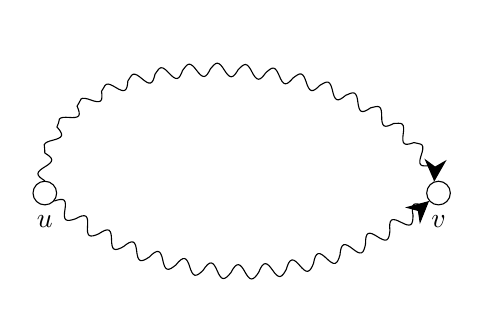
\begin{tikzpicture}
		\node[vert,label=below:$u$] (u) at (1,0) {};
		\node[vert,label=below:$v$] (v) at (6,0) {};
		
		\draw [dirwave] (u) to [out=90,in=110] (v);
		\draw [dirwave] (u) to [out=320,in=220] (v);
		
	\end{tikzpicture}

	%%G2
	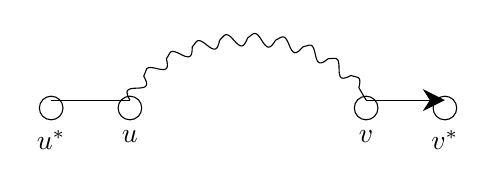
\begin{tikzpicture}
		\node[vert,label=below:$u^*$] (u*) at (1,0) {};
		\node[vert,label=below:$u$] (u) at (2,0) {};
		\node[vert,label=below:$v$] (v) at (5,0) {};
		\node[vert,label=below:$v^*$] (v*) at (6,0) {};
		
		%\draw (u*) -- (u) (v*) -- (v);
		
		%\draw [wave] (u*) to [out=320,in=220] (v*);
		\draw [transform canvas={yshift=1mm}] 
		(1,0) -- (2,0) 
		(2,0) edge[wave] [out=60,in=120] (5,0) 
		(5,0) edge[diredge2] (6,0);
		
	\end{tikzpicture}

	%%G4
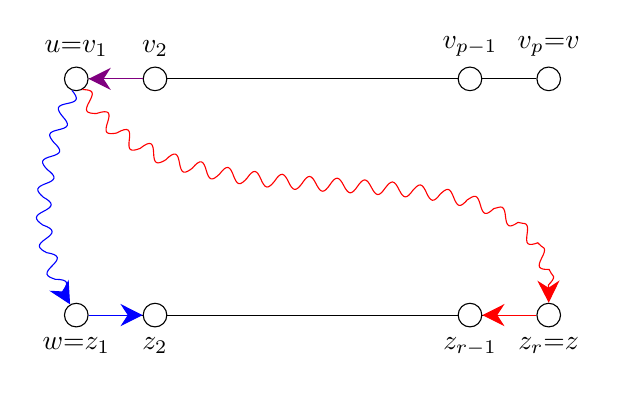
\begin{tikzpicture}
	%%%S_uv
\node[vert,label=above:$u {=} v_1$] (v1) at (1,0) {};
\node[vert,label=above:$v_2$] (v2) at (2,0) {};
\node[vert,label=above:$v_{p-1}$] (vp1) at (6,0) {};
\node[vert,label=above:$v_p {=} v$] (vp) at (7,0) {};
\draw (v1) -- (v2) -- (vp1) -- (vp);

%%%% S_wz
\node[vert,label=below:$w {=} z_1$] (z1) at (1,-3) {};
\node[vert,label=below:$z_2$] (z2) at (2,-3) {};
\node[vert,label=below:$z_{r-1}$] (zr1) at (6,-3) {};
\node[vert,label=below:$z_r {=} z$] (zr) at (7,-3) {};
\draw (z1) -- (z2) -- (zr1) -- (zr);


\draw [violet] (v2) edge[diredge2] (v1);

\draw [blue]%[transform canvas={yshift=0.5mm},thick] 
(v1) edge[dirwave] [out=250,in=120] (z1) 
(z1) edge[diredge2] (z2);


\draw [red] %[transform canvas={yshift=-0.5mm}] 
(v1) edge[dirwave] [out=300,in=90] (zr) 
(zr) edge[diredge2] (zr1);
\end{tikzpicture}

	%%G5
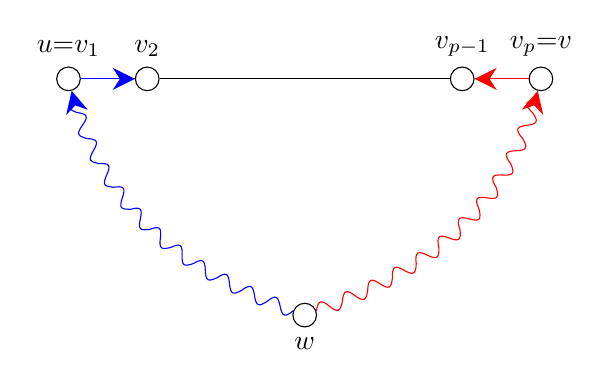
\begin{tikzpicture}
	%%%S_uv
	\node[vert,label=above:$u {=} v_1$] (v1) at (1,0) {};
	\node[vert,label=above:$v_2$] (v2) at (2,0) {};
	\node[vert,label=above:$v_{p-1}$] (vp1) at (6,0) {};
	\node[vert,label=above:$v_p {=} v$] (vp) at (7,0) {};
	\draw (v1) -- (v2) -- (vp1) -- (vp);
	
	%%%% node w
	\node[vert,label=below:$w$] (w) at (4,-3) {};
	
	
	
	\draw [blue]%[transform canvas={yshift=0.5mm},thick] 
	(w) edge[dirwave] [out=160,in=285] (v1) 
	(v1) edge[diredge2] (v2);
	
	\draw [red]%[transform canvas={yshift=0.5mm},thick] 
	(w) edge[dirwave] [out=20,in=255] (vp) 
	(vp) edge[diredge2] (vp1);
	
	
\end{tikzpicture}

	%%G6
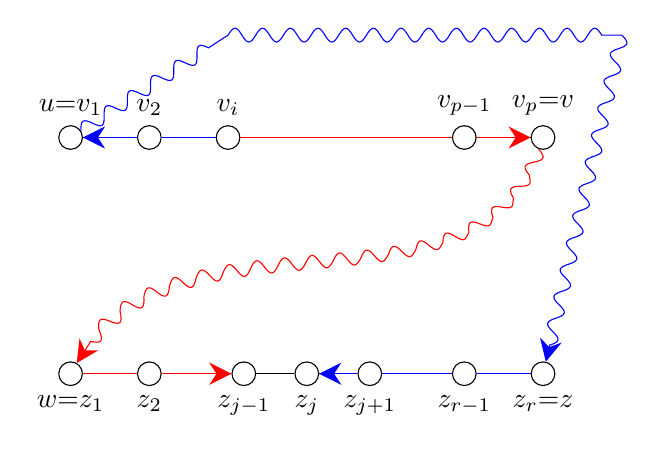
\begin{tikzpicture}
	%%%S_uv
	\node[vert,label=above:$u {=} v_1$] (v1) at (1,0) {};
	\node[vert,label=above:$v_2$] (v2) at (2,0) {};
	\node[vert,label=above:$v_i$] (vi) at (3,0) {};
	\node[vert,label=above:$v_{p-1}$] (vp1) at (6,0) {};
	\node[vert,label=above:$v_p {=} v$] (vp) at (7,0) {};
	\draw (v1) -- (v2) -- (vi) -- (vp1) -- (vp);
	
	%%%% S_wz
	\node[vert,label=below:$w {=} z_1$] (z1) at (1,-3) {};
	\node[vert,label=below:$z_2$] (z2) at (2,-3) {};
	\node[vert,label=below:$z_{j-1}$] (zj-1) at (3.2,-3) {};
	\node[vert,label=below:$z_{j}$] (zj) at (4,-3) {};
	\node[vert,label=below:$z_{j+1}$] (zj+1) at (4.8,-3) {};
	\node[vert,label=below:$z_{r-1}$] (zr1) at (6,-3) {};
	\node[vert,label=below:$z_r {=} z$] (zr) at (7,-3) {};
	\draw (z1) -- (z2) -- (zj-1) -- (zj) -- (zj+1) -- (zr1) -- (zr);
	
	
	
	\draw [blue]%[transform canvas={yshift=0.5mm},thick] 
	(vi) -- (v2) edge[diredge2] (v1) 
	(v1) edge[wave] (3,1.3) 
	(3,1.3) edge[wave] (8,1.3)
	(8,1.3) edge[dirwave] (zr) 
	(zr) --(zr1) -- (zj+1)
	(zj+1) edge[diredge2] (zj);
	
	\draw [red]
	(vi) -- (vp1) edge[diredge2] (vp) 
	(vp) edge[dirwave] [out=250,in=60] (z1) 
	(z1) --(z2)
	(z2) edge[diredge2] (zj-1);
	

\end{tikzpicture}

	%%G7
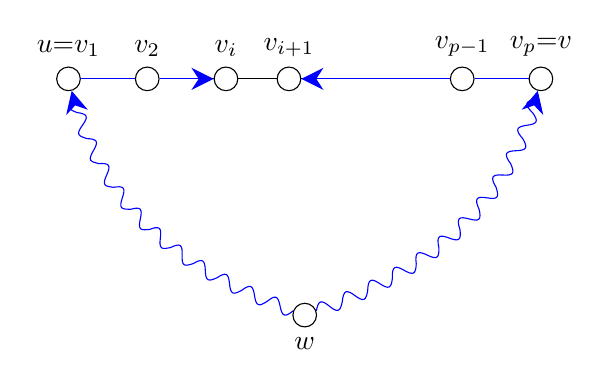
\begin{tikzpicture}
	%%%S_uv
	\node[vert,label=above:$u {=} v_1$] (v1) at (1,0) {};
	\node[vert,label=above:$v_2$] (v2) at (2,0) {};
	\node[vert,label=above:$v_i$] (vi) at (3,0) {};
	\node[vert,label=above:$v_{i+1}$] (vi+1) at (3.8,0) {};
	\node[vert,label=above:$v_{p-1}$] (vp1) at (6,0) {};
	\node[vert,label=above:$v_p {=} v$] (vp) at (7,0) {};
	\draw (v1) -- (v2) -- (vi) -- (vi+1) -- (vp1) -- (vp);
	
	%%%% node w
	\node[vert,label=below:$w$] (w) at (4,-3) {};
	
	
	
	\draw [blue] 
	(w) edge[dirwave] [out=160,in=285] (v1) 
	(v1) -- (v2)
	(v2) edge[diredge2] (vi);
	
	\draw [blue]
	(w) edge[dirwave] [out=20,in=255] (vp) 
	(vp) -- (vp1)
	(vp1) edge[diredge2] (vi+1);
	
	
\end{tikzpicture}

	%%G8
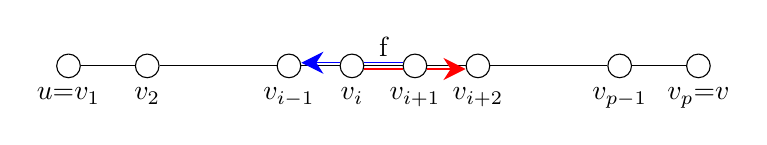
\begin{tikzpicture}
	%%%S_uv
	\node[vert,label=below:$u {=} v_1$] (v1) at (1,0) {};
	\node[vert,label=below:$v_2$] (v2) at (2,0) {};
	\node[vert,label=below:$v_{i-1}$] (vi-1) at (3.8,0) {};
	\node[vert,label=below:$v_{i}$] (vi) at (4.6,0) {};
	\node[vert,label=below:$v_{i+1}$] (vi+1) at (5.4,0) {};
	\node[vert,label=below:$v_{i+2}$] (vi+2) at (6.2,0) {};
	\node[vert,label=below:$v_{p-1}$] (vp1) at (8,0) {};
	\node[vert,label=below:$v_p {=} v$] (vp) at (9,0) {};
	\draw (v1) -- (v2)  -- (vi-1) -- (vi) -- (vi+1) -- (vi+2) -- (vp1) -- (vp);
	\path (vi) -- (vi+1) node [midway,above] {f};	
	
	
	
	\draw [blue,transform canvas={yshift=0.4mm}] 
	(vi+1) -- (vi)
	(vi) edge[diredge2] (vi-1);
	
	\draw [red,transform canvas={yshift=-0.4mm}] 
	(vi) -- (vi+1)
	(vi+1) edge[diredge2] (vi+2);
	

	
	
\end{tikzpicture}

\clearpage

\begin{figure}
	\begin{subfigure}{0.48\textwidth}
		\centering
		\resizebox{\linewidth}{!}{
		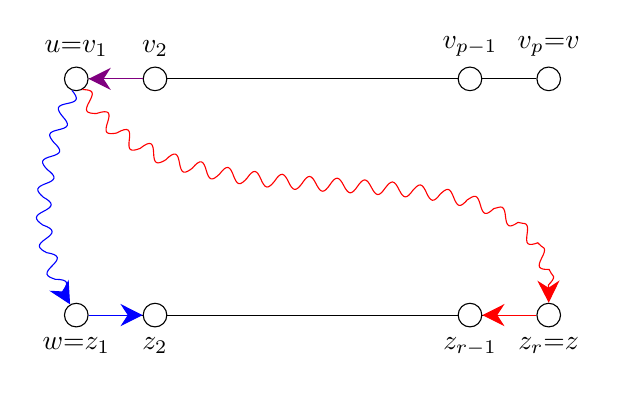
\begin{tikzpicture}
			%%%S_uv
			\node[vert,label=above:$u {=} v_1$] (v1) at (1,0) {};
			\node[vert,label=above:$v_2$] (v2) at (2,0) {};
			\node[vert,label=above:$v_{p-1}$] (vp1) at (6,0) {};
			\node[vert,label=above:$v_p {=} v$] (vp) at (7,0) {};
			\draw (v1) -- (v2) -- (vp1) -- (vp);
			
			%%%% S_wz
			\node[vert,label=below:$w {=} z_1$] (z1) at (1,-3) {};
			\node[vert,label=below:$z_2$] (z2) at (2,-3) {};
			\node[vert,label=below:$z_{r-1}$] (zr1) at (6,-3) {};
			\node[vert,label=below:$z_r {=} z$] (zr) at (7,-3) {};
			\draw (z1) -- (z2) -- (zr1) -- (zr);
			
			
			\draw [violet] (v2) edge[diredge2] (v1);
			
			\draw [blue]%[transform canvas={yshift=0.5mm},thick] 
			(v1) edge[dirwave] [out=250,in=120] (z1) 
			(z1) edge[diredge2] (z2);
			
			
			\draw [red] %[transform canvas={yshift=-0.5mm}] 
			(v1) edge[dirwave] [out=300,in=90] (zr) 
			(zr) edge[diredge2] (zr1);
		\end{tikzpicture}}
	\caption{Example of a guess G-4, where we guessed the fastest temporal paths of form $v_2 \rightarrow u \leadsto w \rightarrow z_2$ (in blue)
	and $v_2 \rightarrow u \leadsto z \rightarrow z_{r-1}$ (in red).
	\label{fig:FPT-guessG4}}
	\end{subfigure}
	\qquad
	\begin{subfigure}{0.48\textwidth}
		\centering
		\resizebox{\linewidth}{!}{
			
			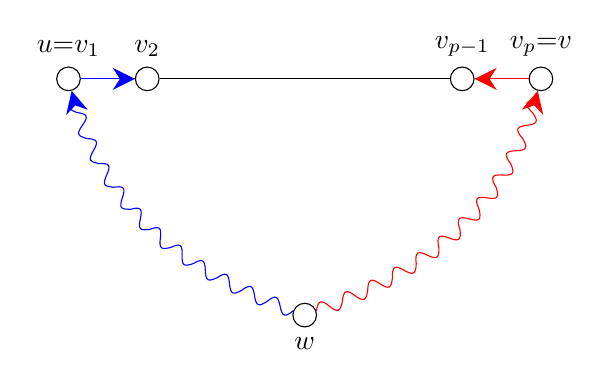
\begin{tikzpicture}
				%%%S_uv
				\node[vert,label=above:$u {=} v_1$] (v1) at (1,0) {};
				\node[vert,label=above:$v_2$] (v2) at (2,0) {};
				\node[vert,label=above:$v_{p-1}$] (vp1) at (6,0) {};
				\node[vert,label=above:$v_p {=} v$] (vp) at (7,0) {};
				\draw (v1) -- (v2) -- (vp1) -- (vp);
				
				%%%% node w
				\node[vert,label=below:$w$] (w) at (4,-3) {};
				
				
				
				\draw [blue]%[transform canvas={yshift=0.5mm},thick] 
				(w) edge[dirwave] [out=160,in=285] (v1) 
				(v1) edge[diredge2] (v2);
				
				\draw [red]%[transform canvas={yshift=0.5mm},thick] 
				(w) edge[dirwave] [out=20,in=255] (vp) 
				(vp) edge[diredge2] (vp1);
				
				
			\end{tikzpicture}}
		\caption{Example of a guess G-5, where we guessed the fastest temporal paths of form $w \leadsto u \rightarrow v_2$ (in blue) and $w \leadsto v \rightarrow v_{p-1}$ (in red). 
			\label{fig:FPT-guessG5}}
	\end{subfigure}
	%
	\begin{subfigure}{0.48\textwidth}
		\centering
		\resizebox{\linewidth}{!}{
			
		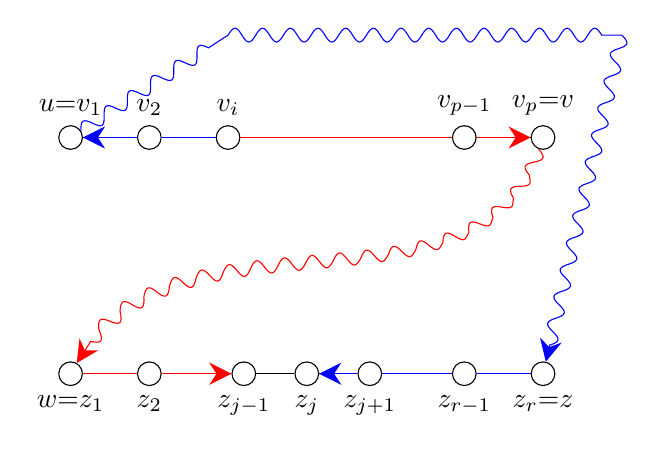
\begin{tikzpicture}
			%%%S_uv
			\node[vert,label=above:$u {=} v_1$] (v1) at (1,0) {};
			\node[vert,label=above:$v_2$] (v2) at (2,0) {};
			\node[vert,label=above:$v_i$] (vi) at (3,0) {};
			\node[vert,label=above:$v_{p-1}$] (vp1) at (6,0) {};
			\node[vert,label=above:$v_p {=} v$] (vp) at (7,0) {};
			\draw (v1) -- (v2) -- (vi) -- (vp1) -- (vp);
			
			%%%% S_wz
			\node[vert,label=below:$w {=} z_1$] (z1) at (1,-3) {};
			\node[vert,label=below:$z_2$] (z2) at (2,-3) {};
			\node[vert,label=below:$z_{j-1}$] (zj-1) at (3.2,-3) {};
			\node[vert,label=below:$z_{j}$] (zj) at (4,-3) {};
			\node[vert,label=below:$z_{j+1}$] (zj+1) at (4.8,-3) {};
			\node[vert,label=below:$z_{r-1}$] (zr1) at (6,-3) {};
			\node[vert,label=below:$z_r {=} z$] (zr) at (7,-3) {};
			\draw (z1) -- (z2) -- (zj-1) -- (zj) -- (zj+1) -- (zr1) -- (zr);
			
			
			
			\draw [blue]%[transform canvas={yshift=0.5mm},thick] 
			(vi) -- (v2) edge[diredge2] (v1) 
			(v1) edge[wave] (3,1.3) 
			(3,1.3) edge[wave] (8,1.3)
			(8,1.3) edge[dirwave] (zr) 
			(zr) --(zr1) -- (zj+1)
			(zj+1) edge[diredge2] (zj);
			
			\draw [red]
			(vi) -- (vp1) edge[diredge2] (vp) 
			(vp) edge[dirwave] [out=250,in=60] (z1) 
			(z1) --(z2)
			(z2) edge[diredge2] (zj-1);
			
			
		\end{tikzpicture}}
		\caption{Example of a guess G-6, where, for fixed a vertex $v_i \in S_{u,v}$,
		we calculated its corresponding split vertex $z_j \in S_{w,z}$,
		and guessed the fastest paths of form
		$v_i \rightarrow v_{i-1} \rightarrow \cdots \rightarrow u \leadsto z \rightarrow z_{r-1} \cdots \rightarrow z_j$ (in blue) 
		and $v_i \rightarrow v_{i+1} \rightarrow \cdots \rightarrow v \leadsto w \rightarrow z_2 \rightarrow \cdots \rightarrow z_{j-1}$ (in red). 
			\label{fig:FPT-guessG6}}
	\end{subfigure}
	\qquad
	\begin{subfigure}{0.48\textwidth}
		\centering
		\resizebox{\linewidth}{!}{
		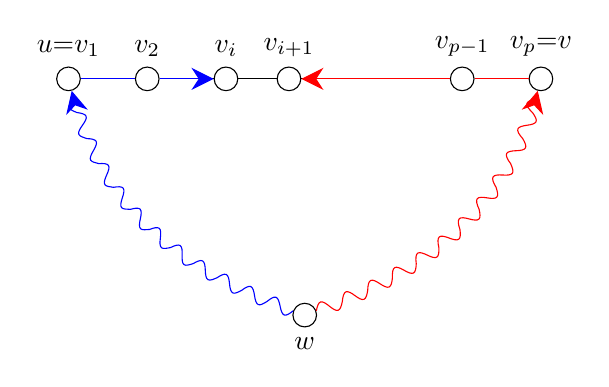
\begin{tikzpicture}
			%%%S_uv
			\node[vert,label=above:$u {=} v_1$] (v1) at (1,0) {};
			\node[vert,label=above:$v_2$] (v2) at (2,0) {};
			\node[vert,label=above:$v_i$] (vi) at (3,0) {};
			\node[vert,label=above:$v_{i+1}$] (vi+1) at (3.8,0) {};
			\node[vert,label=above:$v_{p-1}$] (vp1) at (6,0) {};
			\node[vert,label=above:$v_p {=} v$] (vp) at (7,0) {};
			\draw (v1) -- (v2) -- (vi) -- (vi+1) -- (vp1) -- (vp);
			
			%%%% node w
			\node[vert,label=below:$w$] (w) at (4,-3) {};
			
			
			
			\draw [blue] 
			(w) edge[dirwave] [out=160,in=285] (v1) 
			(v1) -- (v2)
			(v2) edge[diredge2] (vi);
			
			\draw [red]
			(w) edge[dirwave] [out=20,in=255] (vp) 
			(vp) -- (vp1)
			(vp1) edge[diredge2] (vi+1);
			
		\end{tikzpicture}}
	\caption{Example of a guess G-7, where, for a vertex of interest $w$, 
		we
		calculated its corresponding split vertex $v_i \in S_{u,v}$,
		and guessed the fastest paths of form
		$w \leadsto u \rightarrow v_2 \rightarrow \cdots \rightarrow v_i$  (in blue) 
		and $w \leadsto v \rightarrow v_{p-1} \rightarrow \cdots \rightarrow v_{i+1}$ (in red). 
		\label{fig:FPT-guessG7}}
	\end{subfigure}
\caption{An example of guesses G-4, G-5, G-6 and G-7.}
\end{figure}


\end{document}